\chapter{Implementación y pruebas del sistema}
\label{chap:implementacion-pruebas}

Este capítulo documenta la ejecución del sistema desarrollado, su trazabilidad y las pruebas de sus cálculos e integración. Se apoya en la arquitectura del capítulo 5 y los métodos de los capítulos 6 a 9. La evaluación con videos experimentales corresponde al capítulo 11.

\section{Entorno de implementación y dependencias}

La implementación utiliza Python 3.12 y bibliotecas especializadas para inferencia, procesamiento de video, cálculo numérico y visualización. El Cuadro~\ref{tab:entorno-implementacion} reúne las dependencias principales del entorno de referencia en CPU. Las versiones se fijan en archivos de dependencias para reducir las variaciones introducidas por actualizaciones del software.

\begin{table}[htbp]
 \centering
 \caption{Dependencias principales del entorno de referencia.}
 \label{tab:entorno-implementacion}
 \small
 \begin{tabularx}{\textwidth}{@{}l l X@{}}
  \toprule
  Componente & Versión & Función \\
  \midrule
  Python & 3.12.x & Ejecución del sistema. \\
  NumPy & 2.2.6 & Operaciones numéricas sobre posiciones y series. \\
  Matplotlib & 3.10.8 & Generación de gráficos. \\
  OpenCV & 4.11.0.86 & Lectura y escritura de video. \\
  PyTorch / Torchvision & 2.7.1 / 0.22.1 (CPU) & Soporte de inferencia. \\
  Ultralytics & 8.3.213 & Detección y seguimiento. \\
  pytest & 9.1.1 & Ejecución de pruebas automatizadas. \\
  \bottomrule
 \end{tabularx}
\end{table}

Colab utiliza un perfil separado, con el PyTorch y el acelerador disponibles en ese servicio. La GPU NVIDIA T4 del entrenamiento descrito en el capítulo 6 no es un requisito de toda ejecución posterior.

Una utilidad comprueba Python, dependencias y, opcionalmente, existencia y extensiones de las entradas externas. No certifica el contenido del video, la adecuación de los pesos ni la validez de las anotaciones.

\section{Integración y ejecución del procesamiento}

El procesamiento general se invoca desde Python mediante la función \texttt{process\_video\_general}. Recibe las rutas del video y los pesos, el directorio de salida y las opciones de análisis. Las entradas se conservan fuera del código: utilizar otro video o modelo no requiere modificar las funciones de cálculo.

La función coordina el seguimiento, el filtrado y los productos solicitados. Devuelve el diccionario de trayectorias, incluso al habilitar la clasificación o los gráficos. Las interfaces de inspección reutilizan ese diccionario para consultar métricas y generar productos individuales sin repetir la inferencia.

Activar la clasificación no obliga a guardarla, y solicitar su guardado sin habilitarla no produce el archivo. El video anotado de Ultralytics utiliza el destino de esa biblioteca, independiente del directorio general de salida. Las pruebas de integración y de salidas comprueban estas condiciones y la propagación de parámetros.

\section{Validación de entradas y tratamiento de errores}

El punto de entrada rechaza una frecuencia de análisis no positiva y los modos de eje temporal no admitidos. La selección de trayectorias también rechaza nombres de filtro desconocidos. Las funciones que requieren intervalos temporales comprueban el orden de las observaciones antes de operar: cuadros repetidos o decrecientes producen una excepción. Los gaps válidos conservan sus índices originales, de acuerdo con el capítulo~\ref{chap:seguimiento}.

Se distinguen tres situaciones. Un valor cero representa una magnitud calculable cuyo resultado es nulo; \texttt{None} representa una magnitud no definida o no calculable; una excepción señala que la entrada incumple una condición requerida. Por ejemplo, una trayectoria estacionaria puede tener rapidez cero y rectitud no definida. Una trayectoria de una sola observación no aporta segmentos para calcular rapidez y las funciones correspondientes devuelven series vacías. El tratamiento concreto depende de la operación solicitada.

Las comprobaciones se aplican en los componentes que consumen los datos, sin validación exhaustiva anticipada. Los errores de seguimiento o escritura que se propagan interrumpen el procesamiento. Pueden quedar productos parciales; no se garantiza un informe de error persistente ni la eliminación de archivos anteriores.

\section{Trazabilidad y reproducibilidad}

Al completar el flujo, se escribe \texttt{run\_metadata.json}. El archivo registra las rutas del video y del modelo, los umbrales de detección, los FPS de análisis, los parámetros analíticos, el filtro y las opciones activadas. También incluye fecha, plataforma, versión de Python y versiones de las bibliotecas principales. Cuando la información está disponible, registra la revisión del código y si existen cambios locales; los campos que no pueden recuperarse permanecen nulos.

Los metadatos no contienen las trayectorias ni las series calculadas. Las marcas de salida indican productos solicitados, sin comprobar todos los archivos generados. El estado de éxito indica que el flujo llegó a escribir los metadatos; no certifica la calidad científica de los resultados.

El registro no calcula huellas de los pesos y del video: sus rutas no verifican la identidad del contenido. Tampoco conserva todos los parámetros del clasificador ni el estado completo del acelerador. Repetir un análisis exige conservar entradas, configuración y versión de implementación. El entorno fijado facilita esa tarea, sin garantizar resultados idénticos entre plataformas o dispositivos.

\section{Estrategia de pruebas automatizadas}

Las pruebas numéricas comparan resultados con valores deducidos independientemente para entradas sencillas. Las de contratos comprueban interfaces, valores predeterminados, retornos y errores esperados. Las de regresión conservan comportamientos establecidos, sin demostrar su adecuación para cualquier situación experimental.

Las pruebas de integración verifican la coordinación entre seguimiento, selección, análisis, clasificación y metadatos. Para ejecutarlas sin pesos ni videos reales se sustituyen componentes por versiones deterministas: el seguimiento entrega trayectorias conocidas y algunas pruebas reemplazan las funciones gráficas por funciones que registran sus llamadas. Otras pruebas examinan la creación efectiva de archivos y las propiedades de las visualizaciones. La sustitución permite aislar errores de integración, pero deja fuera el desempeño real de la inferencia.

La suite incluye además comprobaciones de normalización de anotaciones, cálculo de errores frente a referencias, inventario del conjunto piloto y organización de artefactos. Esas pruebas verifican la infraestructura de evaluación sobre casos controlados; no equivalen a evaluar el sistema con una referencia manual experimental. El Cuadro~\ref{tab:matriz-pruebas} resume casos representativos sin reproducir el inventario completo de archivos.

\begin{table}[htbp]
 \centering
 \caption{Casos representativos de verificación del sistema.}
 \label{tab:matriz-pruebas}
 \footnotesize
 \renewcommand{\arraystretch}{1.12}
 \begin{tabularx}{\textwidth}{@{}p{0.22\textwidth}X X@{}}
  \toprule
  Comportamiento & Entrada controlada & Resultado esperado \\
  \midrule
  Distancias & Dos segmentos perpendiculares de 3 y 4 px. & Distancia acumulada de 7 px y neta de 5 px. \\
  Rapidez con gaps & Desplazamientos e intervalos temporales conocidos. & División por el tiempo real entre observaciones. \\
  Orden temporal & Cuadros repetidos o decrecientes. & Rechazo mediante \texttt{ValueError}. \\
  Casos degenerados & Una observación o posiciones estacionarias. & Series vacías, ceros o magnitudes no definidas según la operación. \\
  Clasificación & Recorridos sintéticos y cantidades de puntos conocidas. & Categorías o estados coherentes con las reglas implementadas. \\
  Integración & Trayectorias deterministas y opciones de procesamiento. & Selección, llamadas, retornos y guardado según la configuración. \\
  Referencias & Predicciones idénticas, desplazadas o incompletas. & Errores y cobertura acordes con el caso construido. \\
  Metadatos & Configuraciones y entornos controlados. & Persistencia de los valores efectivos y campos nulos previstos. \\
  \bottomrule
 \end{tabularx}
\end{table}

\section{Prueba controlada de rapidez con observaciones ausentes}

Para ilustrar una comprobación numérica se utiliza una trayectoria sintética con observaciones en los cuadros 0, 1, 4 y 5. Las posiciones horizontales son 0, 2, 8 y 10 px, respectivamente, y la coordenada vertical es cero. Se fija una frecuencia de análisis de 30 FPS. Los cuadros 2 y 3 no tienen observaciones; no se incorporan posiciones interpoladas.

El resultado esperado es 60 px/s en cada uno de los tres segmentos. En el intervalo que atraviesa el gap, el desplazamiento es de 6 px y el tiempo transcurrido es de $3/30$ s. Por tanto, aplicar la definición del capítulo~\ref{chap:analisis-trayectorias} conserva el mismo valor que en los segmentos de cuadros consecutivos. La prueba detectaría un cálculo que tratara todas las observaciones como consecutivas, porque ese procedimiento alteraría la rapidez del segmento central.

La Figura~\ref{fig:prueba-rapidez-gaps} muestra las entradas y los valores obtenidos al ejecutar la función real de cálculo. La comparación numérica utiliza tolerancias absoluta y relativa de $10^{-12}$; en este caso, los tres errores absolutos son cero. También se comprueba que los valores quedan asociados a los cuadros finales 1, 4 y 5.

\begin{figure}[htbp]
 \centering
 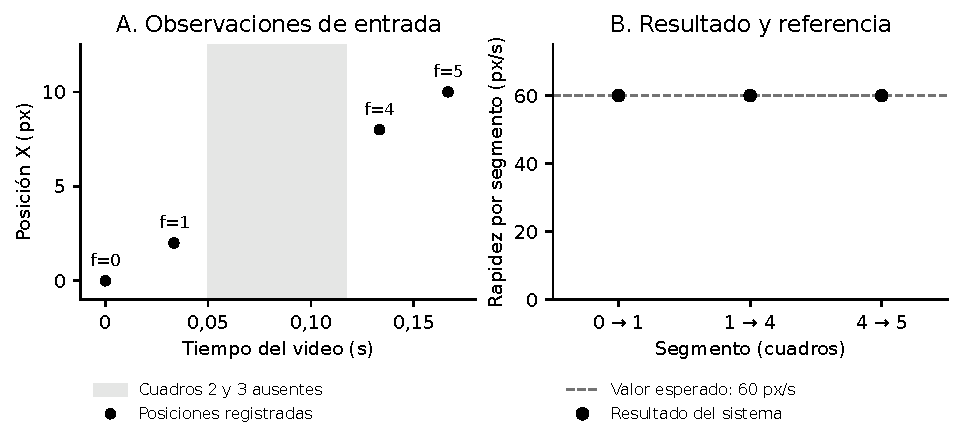
\includegraphics[width=\textwidth]{figures/chapter10/fig10_01_prueba_rapidez_gaps.pdf}
 \caption{Prueba sintética de rapidez con observaciones ausentes. A: posiciones registradas y franja correspondiente a los cuadros 2 y 3 sin observación. B: rapidez calculada para cada segmento y valor esperado. Los resultados coinciden en 60 px/s; cada punto representa una rapidez media entre dos posiciones, no una medición instantánea dentro del intervalo.}
 \label{fig:prueba-rapidez-gaps}
\end{figure}

Un script importa la función del sistema y guarda el gráfico y un registro JSON de entradas, resultados, tolerancias, versiones y huellas de los archivos fuente. La prueba aísla el cálculo de rapidez sin ejecutar el detector; no valida la localización ni reconstruye lo ocurrido dentro del gap.

\section{Alcance de la verificación}

La ejecución de la suite sobre la revisión \texttt{cf1db739a9e2} del sistema finalizó con 381 pruebas aprobadas, sin pruebas omitidas. Se utilizó Linux con Python 3.12.14, NumPy 2.2.6, Matplotlib 3.10.8, OpenCV 4.11.0.86 y pytest 9.1.1. Esta ejecución empleó la sustitución de la interfaz de YOLO prevista en la configuración de pruebas y no instaló PyTorch, Torchvision ni Ultralytics. Por ello, no corresponde a una comprobación del entorno completo de inferencia del Cuadro~\ref{tab:entorno-implementacion}. La prueba ilustrada se ejecutó adicionalmente sobre esa misma revisión.

Los resultados aportan evidencia de consistencia numérica y de integración para los casos cubiertos. No acreditan la exactitud del detector, la conservación de identidad en cruces u oclusiones, la adecuación de los umbrales ni la validez física de las categorías de movimiento. Tampoco establecen tiempos de procesamiento sobre videos reales. Esos aspectos requieren la evaluación experimental del capítulo 11 y deben distinguirse de la aprobación de las pruebas automatizadas.
